\chapter{INTRODUCTION TO PROJECT}
\noindent BlueNRG is a very low power Bluetooth low energy (BLE) single-mode network processor, compliant with Bluetooth specification v4.0. It has an embedded Bluetooth low energy protocol stack: GAP, GATT, SM, L2CAP, LL, RF-PHY. It can play both master and slave roles communicating with other devices or PCs using a proprietary Application Controller Interface (ACI) in addition to the standard Host Controller Interface (HCI) via SPI (Serial Peripheral Interface). 
\section{Overview}
\noindent In order to have two devices communicate with each other using Bluetooth, one needs to ensure that both devices are equipped with the enough hardware capability and apt software support. The fundamental component of a Bluetooth device is the Bluetooth radio and some necessary subset of the Bluetooth stack. BlueNRG is one such device. Like any other Bluetooth hardware device, BlueNRG can be used as an adapter to work with a host system that otherwise does not have the hardware to function Bluetooth. This use case makes BlueNRG a peripheral to a host i.e. A system on chip. \\
\noindent The host system must be able to communicate with BlueNRG in order set straight the relationships and interaction between various portions of the stack. These communications are of course handled by the Operating System. Furthermore for the OS to communicate with an external peripheral, device drivers are employed. And this is the whole idea of this project: creating a device driver for BlueNRG so that it can be used in conjunction with systems running on Linux based operating systems.\\
\noindent The device driver ensures that the peripheral is able to communicate with the host but the way this communication is to be conducted depends on what physical connection options are offered by the peripheral. In case of BlueNRG, the physical interface is SPI. Once the means of communication are fixed, there comes the question of deciding which part of the protocol is to reside on which side, the host or the peripheral. It will be seen in later chapters as to how the whole stack has been fragmented in this project.\\
\noindent Linux is written in C and so are the device drivers for Linux.
\section{Existing Systems}
\noindent Bluetooth has been a prominent technology in networking and has been the backbone of many user applications. As such it only makes sense that an operating system incorporates enough attention to Bluetooth as a technology. And this is exactly the case with Linux. It was realized early on that Bluetooth is going to be a major player and hence efforts were made to have it be an integral part of Linux. The software side of Bluetooth is official Bluetooth protocol stack for Linux which will be looked at in later sections of this report. The other major thing that then remains is the hardware: the Bluetooth adapter. In the modern computers mostly the Bluetooth adapter is inbuilt in the computer hardware itself but even if a Bluetooth adapter is not inbuilt into the system, there are a plethora of very inexpensive Bluetooth adapters in the market that can be used as plug and play peripheral to get Bluetooth working. This is of course possible because Linux, the OS has a stack support for Bluetooth, so once a hardware is detected then all that remains is to bridge this stack to the device using some standard protocol. All of this is taken care by the device driver for that particular device. It is simple, in order for a device to be supported, there has to be a device driver for it, and in this section I describe some of the widely used Bluetooth adapters that are supported by Linux at the time this writing:
\subsection{BlueFritz USB Bluetooth adapter}
The Bluetooth-Stick BlueFRITZ! USB allows you cordless connects to various Bluetooth devices. These can be, for example, access points for DSL or ISDN. It is very apt to connect to printers, mobile phones and PDAs. This allows better mobility, high speed, faster connection set-up and optimal line quality and maximum operational safety.
\begin{figure}[ht]
	\centering
	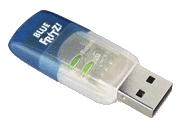
\includegraphics[width=3.5in, height=3in]{images/bluefritz_usb.png}
	\caption{BlueFritz USB Bluetooth Adapter}
\end{figure}
\subsection{Qualcomm Atheros chips}
Qualcomm Atheros is a developer of semiconductors for network communications, particularly wireless chipsets. Qualcomm Atheros offers Bluetooth chips for a variety of platforms. The company also offers integrated combo WLAN and Bluetooth chips. In July 2008, Atheros released an open-source Linux driver for their 802.11n devices which includes its Bluetooth chipset as well. 
\begin{figure}[ht]
	\centering
	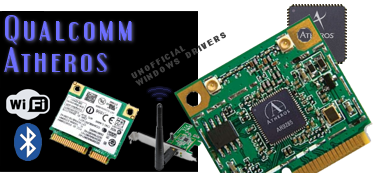
\includegraphics[width=3.5in, height=3in]{images/qualcomm_atheros.png}
	\caption{Qualcomm Atheros chips}
\end{figure}
Qualcomm Atheros’ Bluetooth solution is the AR3001 family of chipsets. The Qualcomm AR3001 is a highly integrated, all-CMOS, single-chip Bluetooth 2.1 and 3.0 + HS solution for mobile handset and portable electronics applications. The compact size and low power consumption of this AR3001 design make it an ideal vehicle for adding Bluetooth to hand-held and other battery-powered consumer electronic devices. The AR3001 supports the standard UART HCI interface and is therefore compatible with any upper layer Bluetooth stack. It is also designed to require less than 12 passive components, thus providing the lowest system BOM cost for mobile phone or portable consumer electronics applications. The AR3001 supports advanced architecture and protocol techniques to save power during sleep, stand-by and active states. The AR3001 family supports 2-, 3- and 4-wire Bluetooth coexistence protocols with advanced algorithms for predicting channel usage by the co-located WLAN transceiver in the same system. It supports all Bluez profiles. 
\subsection{Intel Bluetooth Devices}
Intel is a leading supplier of Bluetooth solutions, offering a product portfolio from mobile phones to automotive, industrial, and medical applications. Linux has drivers for Bluetooth devices offered by Intel.\\
They offer single-chip semiconductor solutions as well as system modules and integrated IP-block solutions to enable increased flexibility and optimization.\\
The Intel BlueMoon architecture is now in its sixth generation and offers a well-proven functionality and performance. Intel BlueMoon products offer superior RF performance along with innovative software solutions for high quality operation. The Intel BlueMoon product family has been designed for voice quality and high-performance data transmissions with reduced requirements on the host processor.\\
Their single solutions are small and cost-effective, targeting mobile phones, automotive, industrial, and medical applications. Intel’s module solutions are Bluetooth qualified, offering an accelerated time to market and lower initial investments.\\
Intel is one of the seven promoters of the Bluetooth SIG and has participated in Bluetooth standardization since the start of Bluetooth.
\begin{figure}[ht]
	\centering
	
\includegraphics[width=3.5in, height=3in]{images/intel_bluetooth.png}
	\caption{Intel Bluetooth Devices}
\end{figure}
\subsection{Broadcom Blutonium}
The Blutonium BCM2045 is the primary single-chip solution for Bluetooth applications, designed from the ground up to promote and enable the adoption of Bluetooth in phones, computers, peripherals and other devices. The chip exhibits stellar features like low power consumption, board space, radio performance and low cost. The chip supports the new Bluetooth Extended Data Rate (EDR), providing raw bandwidth of 3 Megabits per second for wireless applications. In addition, Broadcom’s inConcert interference avoidance technology reduces possible disruption from nearby Wi-Fi products, which operate in the same 2.4 GHz radio frequency as Bluetooth.
\begin{figure}[ht]
	\centering
	
\includegraphics[width=3.5in, height=3in]{images/broadcom_blutonium.png}
	\caption{Broadcom Blutonium}
\end{figure}
\subsection{Marvell Bluetooth}
88W8689 constitutes Marvell’s family of Bluetooth solutions among other solutions as well. With the addition of 88W8689, Marvell now provides a comprehensive set of Bluetooth 2.0-enabled products that target high-volume consumer markets. The highly integrated chip is optimized for both voice and audio transmissions, enabling an array of ultra-mobile, low-power consumer devices. \\
There are other solutions by Marvell for Bluetooth as well and they work well with Linux as the driver is there for them.
\begin{figure}[ht]
	\centering
	
\includegraphics[width=3.5in, height=3in]{images/marvell_bluetooth.png}
	\caption{Marvell Bluetooth}
\end{figure}
\subsection{3Com Bluetooth PCMCIA Card}
The 3Com Wireless Bluetooth PC Card is a Bluetooth version 1.1 device, but 3Com refers it as Version 2.0. Two applications are included: 3Com Bluetooth Mobile Connection Manager, for mobile communications configuration outside the Bluetooth network, and 3Com Bluetooth Connection Manager. The 3Com PC Card adapter provides a well-designed and easy-to-use solution with the antenna retracted, the device sits flush with the edge of your notebook’s Type II PC Card slot, making it easy to transport. You can even leave the PC Card in your notebook permanently so that you’re always prepared to connect with other Bluetooth-enabled devices. While leaving the 3Com card in your computer will cause minimal battery drain, you can always disable the adapter by ejecting it.\\
The PC Card is easy to install and has support in Linux kernel as well.
\begin{figure}[ht]
	\centering
	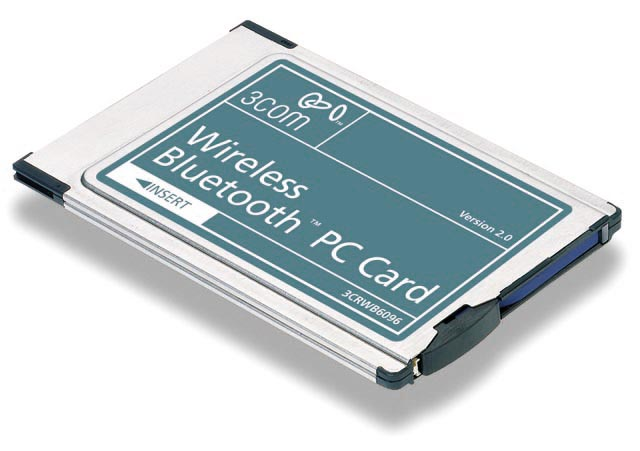
\includegraphics[width=3.5in, height=3in]{images/3com_bluetooth.png}
	\caption{3Com Bluetooth PCMCIA Card}
\end{figure}
\subsection{Texas Instrument Dual-mode Bluetooth CC2564 Module}
The CC2564MODAEM evaluation board contains the Bluetooth BR/EDR/LE HCI solution. Based on TI's CC2564B dual-mode Bluetooth single-chip device, the bCC2564MODA is intended for evaluation and design purposes, reducing design effort and enabling fast time to market. This module has the following set of features:
\begin{itemize}
	\item CC2564MODN device (MOE package)
	\item Bluetooth Specification v4.1
	\item Dual Mode - Bluetooth \& Bluetooth low energy
	\item FCC, IC, CE certified
	\item Class 1.5 Transmit Power (+10dBm)
	\item High sensitivity (-93 dBm typ.)
	\item UART Interface - Control and Data
	\item PCM/I2S Interface - Voice and Audio
	\item 4 Layer PCB design
	\item 1.8 LDO (LP2985-18)
	\item 3 Voltage level translators (SN74AVC4T774)
	\item Chip antenna (LTA-5320-2G4S3-A1) and RF connector (U.FL-R-SMT-1)
	\item EM connectors that plug directly into the TI hardware development kits:
	\begin{itemize}
		\item MSP-EXP430F5529
		\item MSP-EXP430F5438
		\item DK-TM4C123G
		\item DK-TM4C129X
	\end{itemize}
	\item COM connector
	\item Certified and royalty-free TI Bluetooth Stack
\end{itemize}
\section{Requirement Analysis}
There are many Bluetooth adapters out there that have well documented and tested support in Linux based operating systems. Linux being an open source kernel is always inviting people to look into its internal working and stack flow in order to contribute in it.\\
STMicroelectronics excels at grabbing newer opportunities and always be ready with solutions that are on par or even transcends other solutions in the market in a wide range of technologies. The Bluetooth technology is no different. ST has its fair share of Bluetooth modules. Along with the Bluetooth Smart technology, ST has also offered modules that serve complaint to that specification. But thing to be considered here is that even though ST has a wide range of Bluetooth solutions, none has Linux support. \\
So the major requirement of this project was to take a Bluetooth module by ST and add its support to Linux. And again Linux being open source makes the job much simpler. The module that was considered is the BlueNRG module which is Bluetooth 4.0 complaint. This means that it has the much coveted Bluetooth Smart (Low Energy) features. So the whole requirement of this project can be summed up as adding support (writing a device driver) in Linux (because it is open source and one of the most popular OS kernels in the world) for the BTLE module offered by STMicroelectronic i.e. BlueNRG.\\
In order to fulfill the above stated requirement it is essential to look into both sides of the coin: Linux driver development and how is the Bluetooth stack being represented there; and then BlueNRG and what portion of the stack is on it and how much of it is needed in order to work with Linux.\\
The official Bluetooth protocol stack for Linux is Bluez. Bluez is designed in such a way that it offers the HCI interface to any adapter that wish to communicate through it. So for a Bluetooth adapter to be connected to a Linux host, and wanting to utilize the Bluez protocol stack, it needs to extend the HCI interface. And since HCI is also part of the Bluetooth standard, it is not very hard have all Bluetooth devices follow the same protocol. If communication between the host and the controller is to be had using the Bluez protocol stack then it has to happen through the Host Controller Interface as defined in the Bluetooth specification document.\\
Now comes the question of whether BlueNRG is capable of HCI communication, to which the answer is a definite yes. As it will be seen later in this report, BlueNRG is designed to communicate using the Application Controller Interface (ACI), which is a proprietary protocol. But the good news is that ACI is almost a super set of the standard HCI protocol. Since ACI is proprietary and Linux Bluetooth stack offers communication to all devices through only the HCI protocol, it becomes essential to use only the HCI subset available for BlueNRG. Another important point to consider is that how the connection is to be made between the Host (running on Linux) and BlueNRG controller. BlueNRG is based on Serial Peripheral Interface, so that is exactly what is required to be used for the connections. 
\section{Feasibility Study}
As stated in the requirement analysis section, there are two things that are needed to considered here:
\subsection{ Does BlueNRG support what Bluez offers?}
The answer is yes. Bluez interfaces with any device or adapter using the Host Controller Interface which is essentially a protocol standard defined in the Bluetooth specification itself as a means to communicate between the host and the controller. Since BlueNRG is responsive to HCI commands, all seems to be set here. The communication between the host and the controller are to be had through HCI commands (send from the host) and HCI events (generated by the controller in response to the commands send by the host). According to the ACI programing manual, HCI is indeed the subset of ACI. So BlueNRG should be able to respond to HCI commands offered by Bluez of Linux.
\subsection{Does Linux supports what BlueNRG uses to communicate through?}
BlueNRG is based on SPI. Any form of communication between the host and BlueNRG is to be had through the Serial Peripheral Interface. While there isn’t a SPI based Bluetooth driver in Linux at the time of this writing, but there certainly is a rich SPI support in Linux. There are many network drivers that allow the communication between the host and the controller through SPI. So following the same footsteps it should be possible to send commands (HCI) from the host to the controller using SPI.\\
Considering the above things, it seems feasible to write a driver for BlueNRG in Linux. The driver shall essentially act as a bridge between Bluez protocol stack residing partly in the user space and partly in the kernel space of Linux and BlueNRG. Every Bluetooth action that is needed to be performed will be in the form of an HCI command, which is what the driver should expect from Bluez and interface it through SPI to BlueNRG.
\section{Obejectives of the Project}
\begin{itemize}
	\item To setup a Bluetooth driver interface for SPI.
	\item To filter HCI commands to the ones that are supported by BlueNRG.
	\item To interface HCI commands from Bluez stack to BlueNRG.
	\item To map Bluez commands to the BlueNRG functionalities.
\end{itemize}
